\chapter{Validation an algorithm}

\section{Machine learning evaluation}
Machine learning diagnostics are tests that can be run to get to know what is and isn't working with a machine learning algorithm. They also provide guidance as to how performance could be improved. 

\subsection{Evaluating the hypothesis}
The most obvious way to test whether the hypothesis is correct is by dividing the training set into two sets. The first set which should have approximatly 70\% of the samples of the original training set will be used to train the learning algorithm. The other set is used to check whether the output of the learning algorithm is correct. After the algorithm has done its learning with the training set, this check set is thrown into the algorithm. Aftwards the output of the algorithm is compared to the labels of the check set. If the output isn't correct, a test error can be computed. These test errors can be used to compute global error value, which could be calculated by, for example, a mean squared error. This value can be used ito evaluate the hypothesis. \cite{evalml}

\subsection{Model selection algorithm}
\label{modelselection}
To get back to the problem of overfitting, there is another method next to regularisation called model selection. Model selection uses the same principle as mentioned above except it divides the training set into three new sets. A new training set, a cross validation set and a test set. \\\\
The training set is used to actually train the algorithm. The cross validation set is used to compare different algorithms or different models. Different models can be tested and compared to eachother by comparing the cross validation error, the error between the prediction and the actual output from the cross validation set. The testing set is used purely to test the algorithm once the cross validation has been done. It is considered good practice to use seperate sets for cross validation and testing. \cite{wiki}

\subsection{Diagnosing bias vs variance}
High variance means that there is an overfitting problem. High bias on the other hand, is the opposite problem. It means that the hypothesis does not fit the training set at all. There is a relation between the amount of training samples and the training error. With more training data, the training error goes down. \\\\
With a low model complexity, there is a high error for the training set and a high error on the test set. This is a signal there is a underfitting problem or a high bias problem. It does not help to increase the amount of training samples since the model just is not complex enough. \\\\
With a high complexity model, the training set error is very low, but the test set error is very high. This is a signal there is an overfitting problem or a variance problem. This can be seen in Figure~\ref{fig:trainingsamples}. The complexity of the model can be adjusted by changing the amount of features that are being used. \cite{stanford}

\subsection{Learning curves}
\begin{figure}[H]
\centering
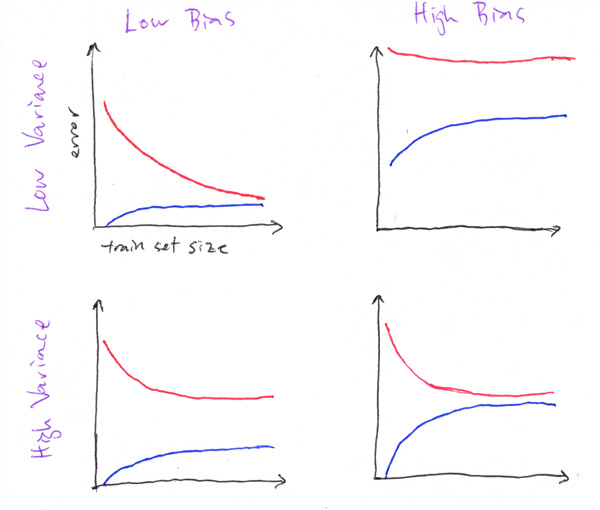
\includegraphics[width=0.8\textwidth]{Figures/bias_variance_chart}
\decoRule
\caption[Training samples comparison]{The effect of the amount of training samples on the accuracy.}
\label{fig:trainingsamples}
\end{figure}
\noindent In Figure~\ref{fig:trainingsamples} the general trend of training error and test (or true) error is shown. This figure shows the example for high bias and no matter how many training samples there are, the functions are already converged to the same error amount.\\\\
In contrary to high bias, high variance can be solved by using extra training samples. In that case there is a gap inbetween the true error line and the training error line and it is likely that they still converge to the same point. With a bigger training set, they converge more and more. These curves are called learning curves.

\section{Error analysis}
When trying to use machine learning for any purpose, such as intrusion detection systems, there are several considerations to be made. Another important step is the approach used to find the correct algorithm. 
The recommended approach is to start with a simple algorithm and test it with cross validation data. Afterwards, learning curves could be plotted to decide if more or less data, more or less features, ... are likely to help. Finally, error analysis can be done by maually examining the samples on which the algorithm made mistakes. This could help to spot any systematic trends in the type of samples on which the algorithm is making mistakes.\\\\
The error analysis mostly consists of manual or brute force work. The samples on which the algorithm is wrong need to be categorized based on which features could help it categorize correctly and on which class it belongs to. Calculating statistics, such as the accuracy of the algorithm can also help with error analysis. It is possible to brute force this approach by automatically trying a lot of different combinations of features. This is less efficient than manually tweaking the algorithm.\\\\
Another issue to account for are skewed classes. Skewed classes are classes that are underrepresented in training data. For example, in binary classification, when trying to classify a flow as malicious or not, the training set might only provide $0.5$\% malicious data. Knowing this, having an accuracy of $99$\% does not seem that great.

\begin{figure}[H]
\centering
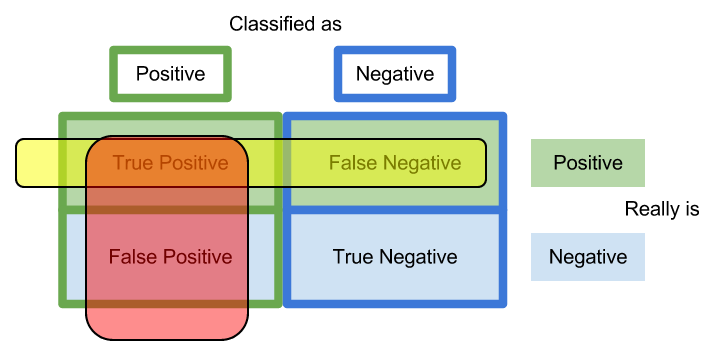
\includegraphics[width=1\textwidth]{Figures/precisionrecall}
\decoRule
\caption[Precision and recall]{Precision and recall. \cite{recall-fig}}
\label{fig:precisionrecall}
\end{figure}
\noindent A different metric is required to evaluate machine learning algorithms that are trained using skewed data. This metric is the precision and recall method. We classify a result as true positive, true negative, false positive and false negative. False positive and false negative respectively mean that the predicted value is falsely classified as positive and negative. These are the errors. True positive and true negative are correctly predicted values. \textbf{Precision} is defined as the fraction of predicted malicious flows that were actually malicious: 
$$\dfrac{true positive}{true positive + false positive}$$
\textbf{Recall} is defined as the fraction of predicted positives and the actual amount of positives: 
$$\dfrac{true positive}{true positive + false negative}$$
There is always a tradeoff to be made between precision and recall. As an effect of a higher precision, there will be a lower recall. Similarly, a higher recall means a lower precision.\\\\
Algorithms with a different precision and recall can be compared to eachother. This can be done using an F-score: 
$$2 \dfrac{PR}{P+R}$$
\noindent The F-score is the harmonic mean of precision and recall. For Table~\ref{tab:precrecal}, this means that Algorithm 1 is the most effective. In contrast, using for example the average of both precision and recall would make Algorithm 3 the most effective.\\\\
The main reason to use the harmonic mean is because the average is taken of
ratios (percentages), and in that case the harmonic mean is more appropriate than the (arithmetic) mean. \cite{harmonic}
\begin{table}[H]
\caption{Example of precision and recall of certain algorithms.}
\label{tab:precrecal}
\centering
\begin{tabular}{| l | c  r|}
\toprule
\tabhead{} & \tabhead{Precision (P)} & \tabhead{Recall (R)}\\
\midrule
Algorithm 1 & 0.5 & 0.4\\
Algorithm 2 & 0.7 & 0.1\\
Algorithm 3 & 0.02 & 1.0\\
\bottomrule
\end{tabular}
\end{table}
\noindent Looking at the values of the precision and the recall in Table~\ref{tab:precrecal}, it can already intuitively be seen that Algorithm 1 is the best algorithm. For algorithm 3, the precision is 0.02, which means that there were a lot more false positives than true positives. With a recall of 1.0, there are almost no false negatives. This means that almost every prediction was a positive. That is not good at all. \\\\
Algorithm 2 has similar problem but the other way around. Only Algorithm 1 seems to have some kind of balance between precision and recall which makes it seem as the best algorithm. This confirms that the F-score is a better metric than the average.
\begin{table}[H]
\caption{Example of average and F-score of certain algorithms.}
\label{tab:avgscore}
\centering
\begin{tabular}{| l | c  r|}
\toprule
\tabhead{} & \tabhead{Average} & \tabhead{F-score}\\
\midrule
Algorithm 1 & 0.45 & 0.444\\
Algorithm 2 & 0.4 & 0.175\\
Algorithm 3 & 0.51 & 0.039\\
\bottomrule
\end{tabular}
\end{table}
\noindent The data that is being fed into a machine learning algorithm is also important to consider. Sometimes a lot of data can be useful. First, the assumption is made that the features are chosen correctly and sufficiently. Lots of data is useful when a machine learning algorithm is used with a lot of parameters such as a neural network with a lot of hidden units. This means that the algorithm has low bias. 

\subsection{Different Algorithms}
If the number of features is large relative to the number of training samples, then using a lineair kernel Support Vector Machine or logistic regression is preferred. A Gaussian kernel is preferred when there are more training samples than features, but the difference is rather small. Otherwise, new features should be added. Neural networks are almost always effective but they may be slower to train.\\\\